\documentclass{article}
\usepackage{geometry}
\usepackage[english]{babel}
\usepackage[utf8]{inputenc}
\usepackage{fancyhdr}
\usepackage{graphicx}
\usepackage{titlesec}
\usepackage{minted}

\setlength{\headheight}{15.2pt}
\setcounter{secnumdepth}{3}
\rfoot{Pg: \thepage}

\geometry{
   a4paper,
   left = 20mm,
   top = 20mm,
}
\begin{document}
\thispagestyle{empty}

\section*{}
{\LARGE\makebox[\textwidth]{\textbf{KATHMANDU UNIVERSITY}}}

\centerline{Department of Computer Science and Engineering}
\centerline{Dhulikhel,Kavre}
\begin{figure}[h]
    \centerline{
\includegraphics[width=50.546mm,height=50.546mm]{KU_Logo.png}}
\end{figure}

\centerline{\textbf{A Project Report}}
\centerline{on}
\centerline{\underline{\textbf{"Sorting techniques and their comparisons in terms of algorithmic complexity"}}}

\vspace*{12mm}

\centerline{\textbf{[Code No. : COMP 202]}}
\centerline{(For partial fulfillment of 2nd Year/ 3rd Semester in Computer Science)}

\vspace*{10mm}

\centerline{\textbf{Submitted by}}
\centerline{\textbf{Aayush Pokharel(Roll No. 43)}}
\centerline{\textbf{Dikshya Poudel (Roll No. 45)}}
\centerline{\textbf{Sajag Pradhanang (Roll No. 47)}}
\centerline{\textbf{Samjhana Bhusal (Roll No. 60)}}

\vspace*{16mm}


\centerline{\textbf{Submitted to}}
\centerline{\textbf{Dr Gajendra Sharma}}
\centerline{\textbf{Dept of Computer Science and Engineering}}

\vspace*{10mm}

\centerline{\textbf{Submission Date: 15th July, 2021}}



\clearpage
\thispagestyle{empty}

\section*{Abstract}
The project ‘Sorting techniques and their comparisons in terms of algorithmic complexity’ 
report is drafted to meet the prerequisites to partially fulfill the COMP 202 course offered 
by the Department of Computer Science and Engineering at Kathmandu University. This project 
is designed to expand the knowledge of various algorithms and their complexity.We, the involved 
project members, have decided to create a report and a github repository with the included 
algorithms that were used in writing this report. The code is in Python language and  is 
platform agnostic. The main goal of this project is to develop an efficient set of python 
code that can we can use as a the basis of argument present herein in this report. We embarked 
in this venture hoping to increase the programming skill of involved project members in hope 
of tackling harder projects in the forthcoming days.

\clearpage
\thispagestyle{empty}
\tableofcontents

\clearpage
\thispagestyle{empty}
\listoffigures

\clearpage
\pagenumbering{arabic}
\section{Introduction to Sorting}
Arranging an unordered sequence into an ordered sequence is called "sorting".
Sorting is a common operation in computer science for many applications, and many different and 
efficient algorithms to perform it have been developed.

\vspace*{5mm}
\subsection{Uses of Sorting}
The most common uses of sorted sequences are:
\begin{itemize}
    \item making lookup or search efficient
    \item making merging of sequences efficient
    \item enable processing of data in a defined order
\end{itemize}

\vspace*{5mm}
\subsection{List of Sorting Algorithms}
Some of the most common sorting algorithms that is used in Computer Science are:
\begin{itemize}
    \item Insertion sort
    \item Bubble sort
    \item Selection sort
    \item Merge sort
    \item Quick sort
    \item Heap sort
\end{itemize}
\clearpage

\section{Algorithm}
There are various algorithms that do sorting through various techniques.
The sorting algorithms present in this report are implemented in python 
programming language for sake of ease due it dynamically typed nature 
and the language's focus on code readability.  

\subsection{Insertation Sort}
\begin{itemize}
    \item \textbf{Time Complexity}
        \begin{itemize}
            \item Best Case: n
            \item Average Case: n\textsuperscript{2}
            \item Worst Case: n\textsuperscript{2}
        \end{itemize}
    \item \textbf{Implementation}
\end{itemize}

\begin{minted}[]{python}
# Code for Insertion Sort
def insertionSort(array):
    for i in range(1, len(array)):      #outside loop. This runs for (n)times
        key = array[i]
        j = i-1
        while j >= 0 and key < array[j] :  #inside loop. This runs for (n-1)times
            array[j + 1] = array[j]
            j -= 1
        array[j + 1] = key
    return array
##
\end{minted}

\begin{itemize}
    \item \textbf{Explaination}
    \begin{itemize}
        \item Insertation sort has two operation.
        \item Scanning through list.
        \item Comparing two elements and changing if out of order.
        \item Scanning is done (n) number of times.
        \item Comparing  and swapping is done (\( \frac{n-1}{2} \)) number of times.
        \item Best case is when a list is in order.
        \item Average in random order 
        \item Worst in opposite order.
        \item In best case only outer loop is triggered. (n) gives \textbf{O(n)}
        \item In Average and Worst Case both loop are triggered. 2n(\( \frac{n-1}{2} \)) gives \textbf{O(n\textsuperscript{2})}
    \end{itemize}
\end{itemize}
\clearpage

\subsection{Bubble Sort}
\begin{itemize}
    \item \textbf{Time Complexity}
        \begin{itemize}
            \item Best Case: n
            \item Average Case: n\textsuperscript{2}
            \item Worst Case: n\textsuperscript{2}
        \end{itemize}
    \item \textbf{Implementation}
\end{itemize}

\begin{minted}[]{python}
# Code for Bubble Sort
def bubbleSort(array):
    n = len(array)

    for i in range(n):      # Outside loop. This runs for (n)times
        swapped = False
        for j in range(0, n-i-1):       # Inside loop
            if array[j] > array[j+1] :  # Only runs if element pair are out of order
                array[j], array[j+1] = array[j+1], array[j] # does (n-1)times of swap
                swapped = True
        if swapped == False:
            break
    return array
##
\end{minted}
\begin{itemize}
    \item \textbf{Explaination}
    \begin{itemize}
        \item scanning is done for (n)times
        \item comparisons then swapping is done (\( \frac{n-1}{2} \))times on average.
        \item when the list is in order only the statement for scanning is executed (n)times which gives \textbf{O(n)}
        \item Otherwise, n(\( \frac{n-1}{2} \)) gives \textbf{O(n\textsuperscript{2})} as n\textsuperscript{2} is highest order of n
    \end{itemize}
\end{itemize}

\clearpage

\subsection{Selection Sort}
\begin{itemize}
    \item \textbf{Time Complexity}
        \begin{itemize}
            \item Best Case: n\textsuperscript{2}
            \item Average Case: n\textsuperscript{2}
            \item Worst Case: n\textsuperscript{2}
        \end{itemize}
    \item \textbf{Implementation}
\end{itemize}

\begin{minted}[]{python}
# Code for Selection Sort
def selectionSort(array):
    for i in range(len(array)): # first loop runs for (n)times
        min_idx = i
        for j in range(i+1, len(array)): # second looop runs for (n-1)times
            if array[min_idx] > array[j]:   # is only executed when pair is out of order
                min_idx = j
    
        array[i], array[min_idx] = array[min_idx], array[i]
    return array
##  
\end{minted}
\begin{itemize}
    \item \textbf{Explaination}
    \begin{itemize}
        \item There are two loops that are used for scanning.
        \item The outr loop runs for (n) times.
        \item The inner loop runs for (n-1) times.
        \item Whether swapping is done or not, the loop for (n) lenght list runs for n(n-1) times.
        \item n(n-1)times gives \textbf{O(n\textsuperscript{2})} as n\textsuperscript{2} is of highest order.
        \end{itemize}
\end{itemize}


\clearpage
\subsection{Merge Sort}
\begin{itemize}
    \item \textbf{Time Complexity}
        \begin{itemize}
            \item Best Case: n log(n)
            \item Average Case: n log(n)
            \item Worst Case: n log (n)
        \end{itemize}
    \item \textbf{Implementation}
\begin{minted}[]{python}
# Code for Merge Sort
def mergeSort(array):
    if len(array) > 1:      
        mid = len(array)//2         
        L = array[:mid]             # the list is always divided in half.
        R = array[mid:]             # it takes constant time

        mergeSort(L)                # they are recursive so they take O(n/2)
        mergeSort(R)                
 
        i = j = k = 0

        while i < len(L) and j < len(R):
            if L[i] < R[j]:
                array[k] = L[i]
                i += 1
            else:
                array[k] = R[j]
                j += 1
            k += 1

        while i < len(L):
            array[k] = L[i]
            i += 1
            k += 1
 
        while j < len(R):
            array[k] = R[j]
            j += 1
            k += 1

    return array                #combining takes (n)times
##
\end{minted}
    \item \textbf{Explaination}
    \begin{itemize}
        \item The division of list takes linear time.
        \item The combination of the list takes (n) times.
        \item The division and combination of list becomes (\textit{c}*n)times. with \textit{c} as some constant.
        \item The two half are called recursively so they take (n/2) times each.
        \item The divisions are exponentially halfed on each call.
        \item The final equation becomes T(n) = 2*T(\( \frac{n}{2} \)) + O(\textit{c}*n)
        \item This gives \textbf{O(n log(n))} for all cases.
    \end{itemize}
\end{itemize}

\clearpage
\subsection{Quick Sort}
\begin{itemize}
    \item \textbf{Time Complexity}
        \begin{itemize}
            \item Best Case: n log (n)
            \item Average Case: n log(n)
            \item Worst Case: n\textsuperscript{2}
        \end{itemize}
    \item \textbf{Implementation}
\begin{minted}[]{python}
#Code for Quick Sort

#function definition of partition function
def partition(start, end, array):
    pivot_index = start
    pivot = array[pivot_index]
    while start < end:                        # k is number of elements less than pivot
        while start < len(array) and array[start] <= pivot: start += 1 # this is done T(k) times
        while array[end] > pivot: end -= 1    # this is done T(n-k-1) times
        if(start < end):
            array[start], array[end] = array[end], array[start]
    array[end], array[pivot_index] = array[pivot_index], array[end]
    return end

# main() function
def quickSort(start, end, array):
    if (start < end):
        p = partition(start, end, array)    # This partitioning gives O(n)
        quickSort(start, p - 1, array)      #   recursive call
        quickSort(p + 1, end, array)        #   recursive call
    return array
##
\end{minted}
    \item \textbf{Explaination}
    \begin{itemize}
        \item The partitioning of list is of linear time and takes \textbf{O(n)}
        \item The partations are divided on a pivot value
        \item In this Implementation of quickSort, the last vale is taken as pivot.
        \item The partations are called recursively.
        \item k is list of value smaller than the pivot.
        \item The smaller partition is of size T(k) which can become T(0) after multiple calls, giving \textbf{O(0)}
        \item The larger is of size T(n-k-1) which gives \textbf{O(n)}
        \item The final equation becomes T(n) = T(n-1) + O(n) giving \textbf{O(n\textsuperscript{2})}
        \item On best case, the eqn becomes T(n) = 2T(n/2) + O(n) due to equal partitions.
        \item This gives \textbf{O(n log(n))}
    \end{itemize}
\end{itemize}

\clearpage
\subsection{Heap Sort}
\begin{itemize}
    \item \textbf{Time Complexity}
        \begin{itemize}
            \item Best Case: n log(n)
            \item Average Case: n log(n)
            \item Worst Case: n log (n)
        \end{itemize}
    \item \textbf{Implementation}
\begin{minted}[]{python}
# Code for Heap Sort

#function definition of heapify function
def heapify(array, n, i):
    largest = i  # Initialize largest as root
    l = 2 * i + 1
    r = 2 * i + 2

    if l < n and array[largest] < array[l]: largest = l
    if r < n and array[largest] < array[r]: largest = r
        
    if largest != i:
        array[i], array[largest] = array[largest], array[i]
        heapify(array, n, largest)    

# main() function
def heapSort(array):
    n = len(array)

    for i in range(n//2 - 1, -1, -1):
        heapify(array, n, i)      

    for i in range(n-1, 0, -1):
        array[i], array[0] = array[0], array[i]
        heapify(array, i, 0)
    return array      
\end{minted}
    \item \textbf{Explaination}
    \begin{itemize}
        \item A maxheap from list is made. This takes \textbf{O(n)}
        \item elements are swapped to make the root largest
        \item the heap decreases and sorted list increases
        \item In each call of recursion, the process is repeated to check the root is still the largest
        \item Thus the heapify() function gives \textbf{O(log(n))}
        \item The final time complexity becomes \textbf{O(n log(n))}
    \end{itemize}
\end{itemize}

\clearpage
\section{Comparision Between Different Sorting Algorithms}
\subsection{Array List code}
\begin{minted}[]{python}
array1 = [1, 2, 3, 4, 5, 6]
array2 = [1, 3, 6, 4, 5, 2]
array3 = [6, 5, 4, 3, 2, 1]
\end{minted}
\subsection{Main Driver Code}
\begin{minted}[]{python}
# This is the code That is kept in main.py file
from ArrayList import *
from sortingTechnique import *
# The individual function definition are in Chapter 2 under their own subsection.

def Driver(array,technique):
    print("The unsorted Array is: ", array)

    if technique == "INSERTION":
        print("The sorted Array is: ", insertionSort(array))
    elif technique == "BUBBLE":
        print("The sorted Array is: ", bubbleSort(array))
    elif technique == "MERGE":
        print("The sorted Array is: ", mergeSort(array))
    elif technique == "SELECTION":
        print("The sorted Array is: ", selectionSort(array))
    elif technique == "QUICK":
    print("The sorted Array with Quick sort is: ", quickSort(0, len(array) - 1, array))
    elif technique == "HEAP":
        print("The sorted Array is: ", heapSort(array))
    else:
        print("Wrong arguments")

if __name__ == "__main__":
    Driver(array1,"INSERTION")
    Driver(array2,"INSERTION")
    Driver(array3,"INSERTION")
    print("\n")
    Driver(array1,"BUBBLE")
    Driver(array2,"BUBBLE")
    Driver(array3,"BUBBLE")
    print("\n")
    Driver(array1,"MERGE")
    Driver(array2,"MERGE")
    Driver(array3,"MERGE")
    print("\n")
    Driver(array1,"SELECTION")
    Driver(array2,"SELECTION")
    Driver(array3,"SELECTION")
    print("\n")
    Driver(array1,"QUICK")
    Driver(array2,"QUICK")
    Driver(array3,"QUICK")
    print("\n")
    Driver(array1,"HEAP")
    Driver(array2,"HEAP")
    Driver(array3,"HEAP")
\end{minted}

\begin{figure}[h]
    \centerline{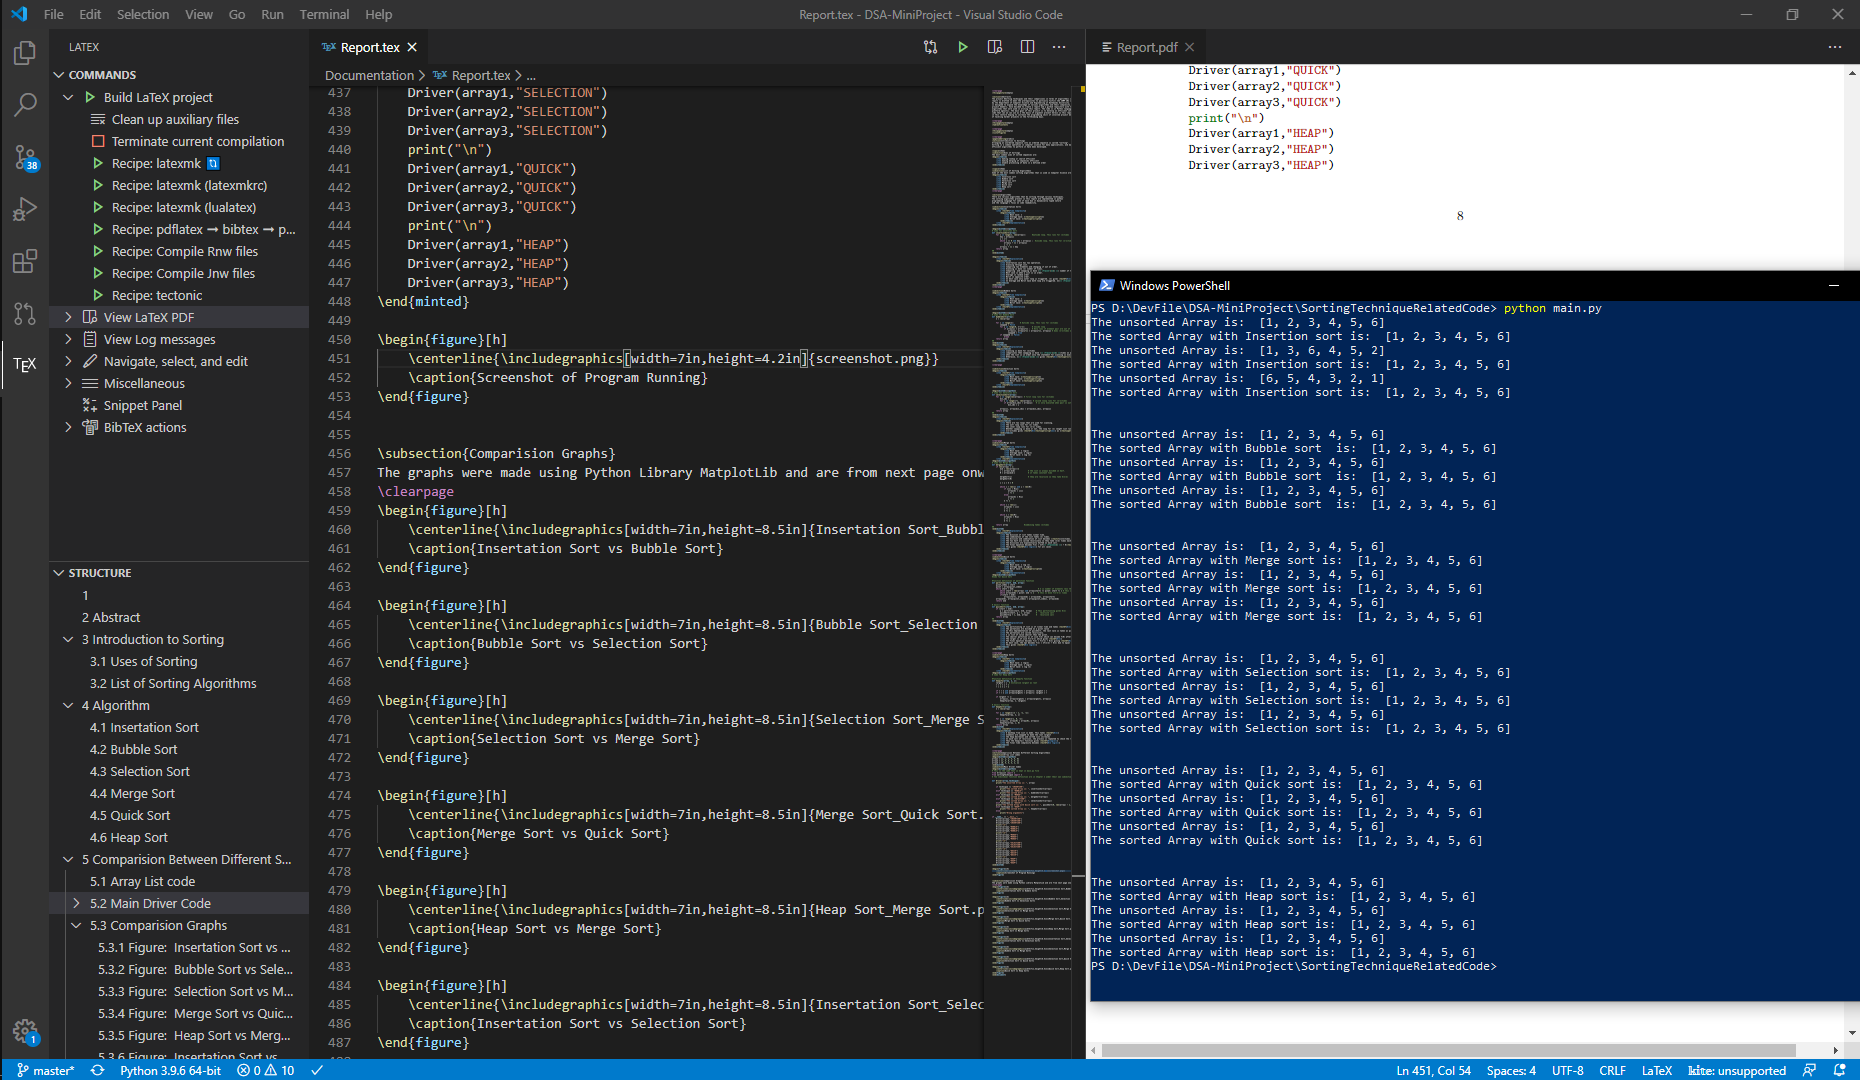
\includegraphics[width=7in,height=4.2in]{screenshot.png}}
    \caption{Screenshot of Program Running}
\end{figure}


\subsection{Comparision Graphs}
The graphs were made using Python Library MatplotLib and are from next page onwards.
\clearpage
\begin{figure}[h]
    \centerline{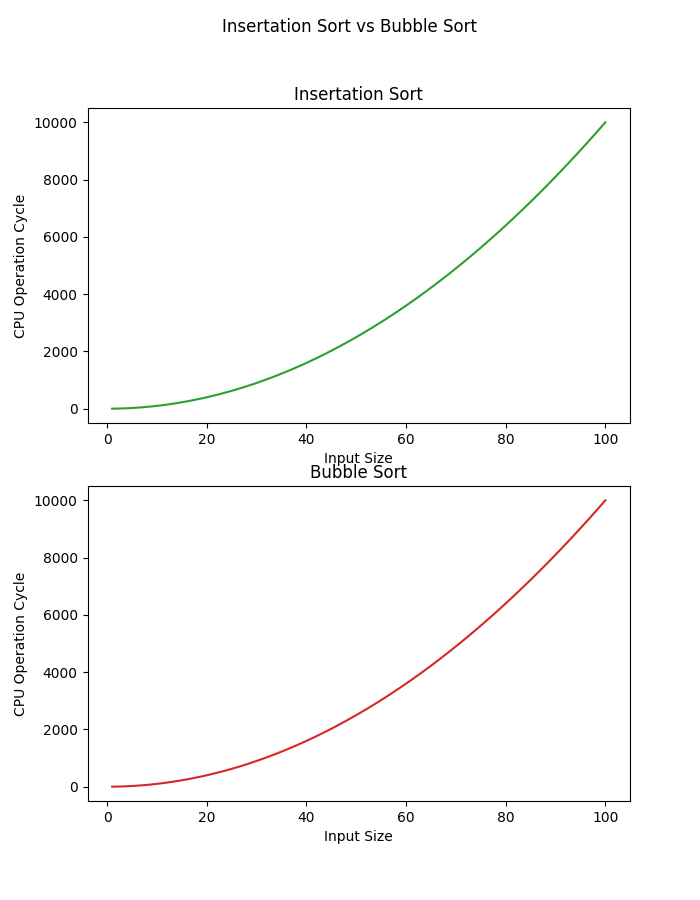
\includegraphics[width=7in,height=8.5in]{Insertation Sort_Bubble Sort.png}}
    \caption{Insertation Sort vs Bubble Sort}
\end{figure}

\begin{figure}[h]
    \centerline{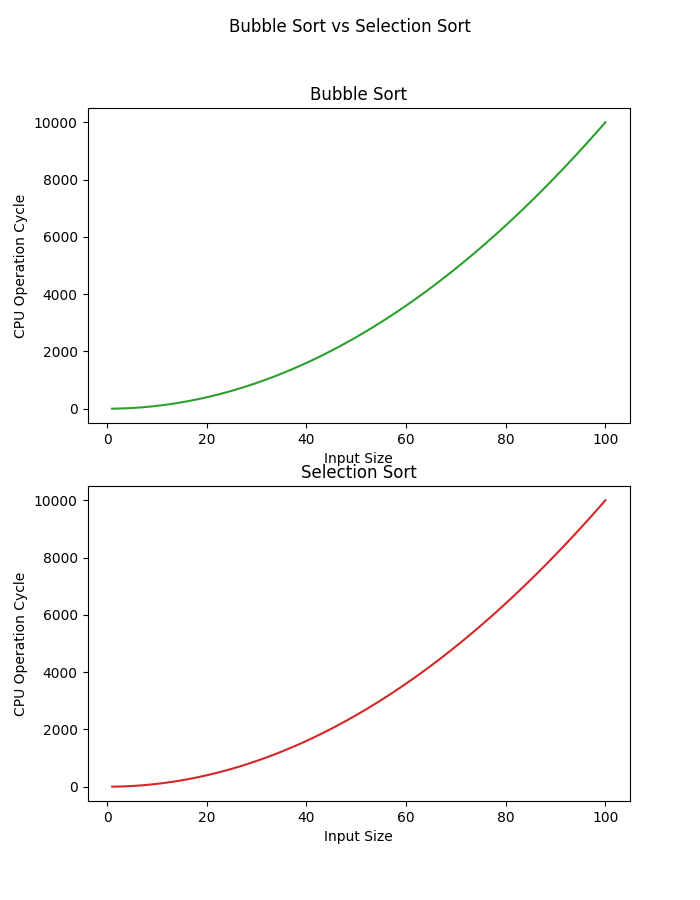
\includegraphics[width=7in,height=8.5in]{Bubble Sort_Selection Sort.png}}
    \caption{Bubble Sort vs Selection Sort}
\end{figure}

\begin{figure}[h]
    \centerline{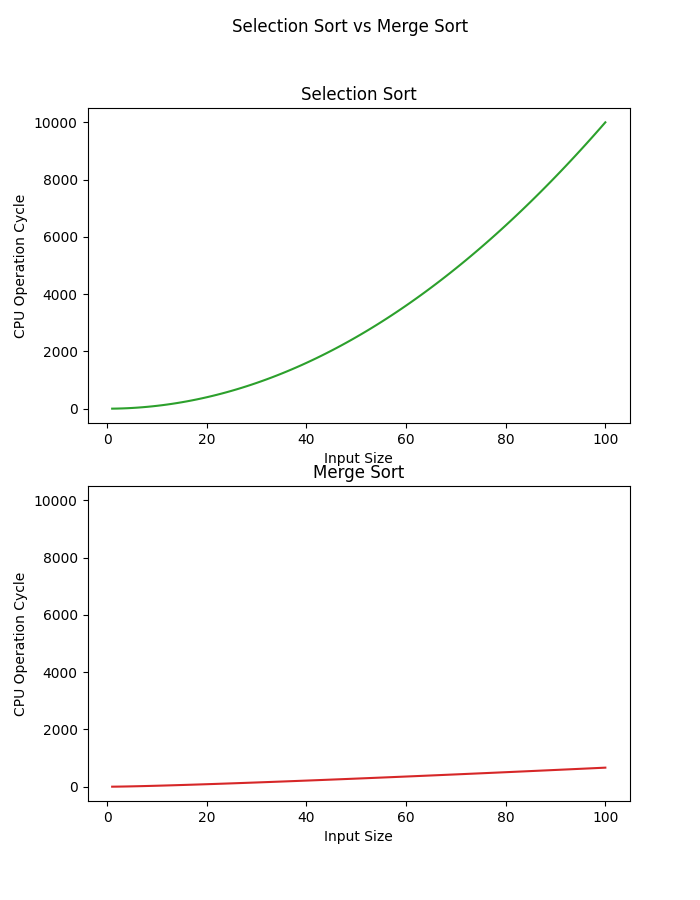
\includegraphics[width=7in,height=8.5in]{Selection Sort_Merge Sort.png}}
    \caption{Selection Sort vs Merge Sort}
\end{figure}

\begin{figure}[h]
    \centerline{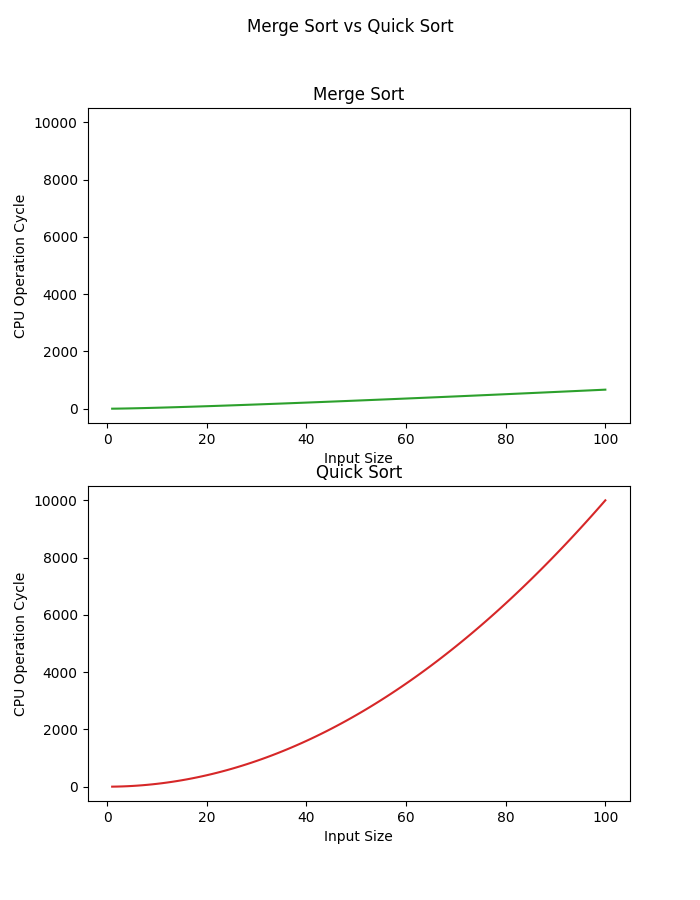
\includegraphics[width=7in,height=8.5in]{Merge Sort_Quick Sort.png}}
    \caption{Merge Sort vs Quick Sort}
\end{figure}

\begin{figure}[h]
    \centerline{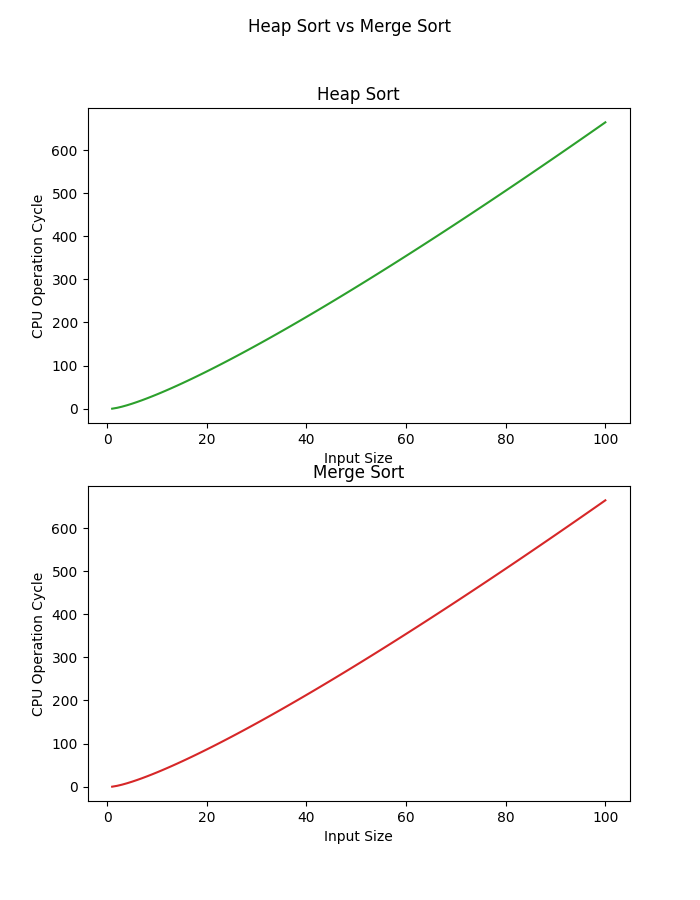
\includegraphics[width=7in,height=8.5in]{Heap Sort_Merge Sort.png}}
    \caption{Heap Sort vs Merge Sort}
\end{figure}

\begin{figure}[h]
    \centerline{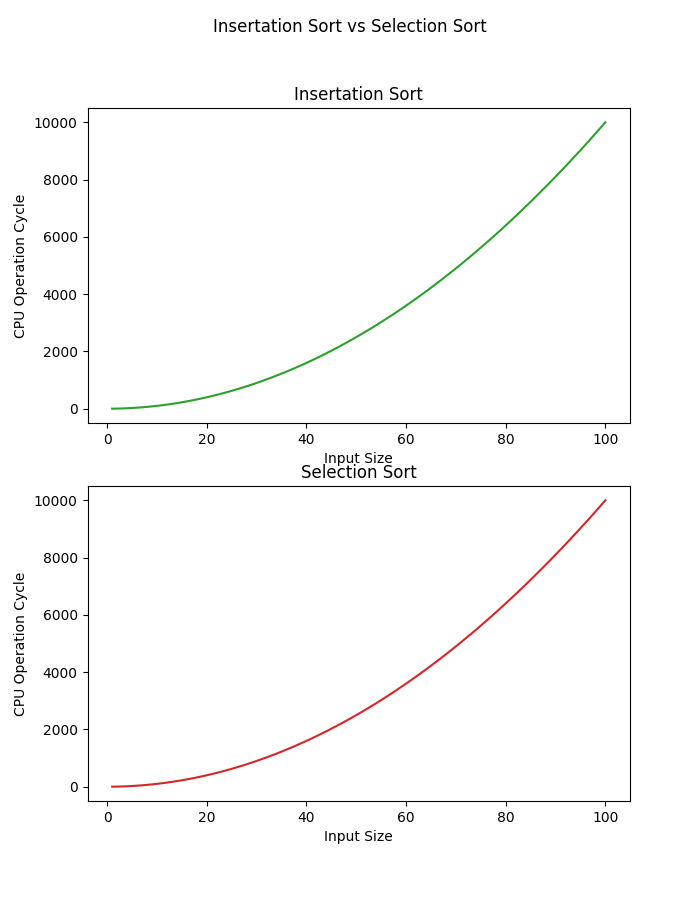
\includegraphics[width=7in,height=8.5in]{Insertation Sort_Selection Sort.png}}
    \caption{Insertation Sort vs Selection Sort}
\end{figure}

\begin{figure}[h]
    \centerline{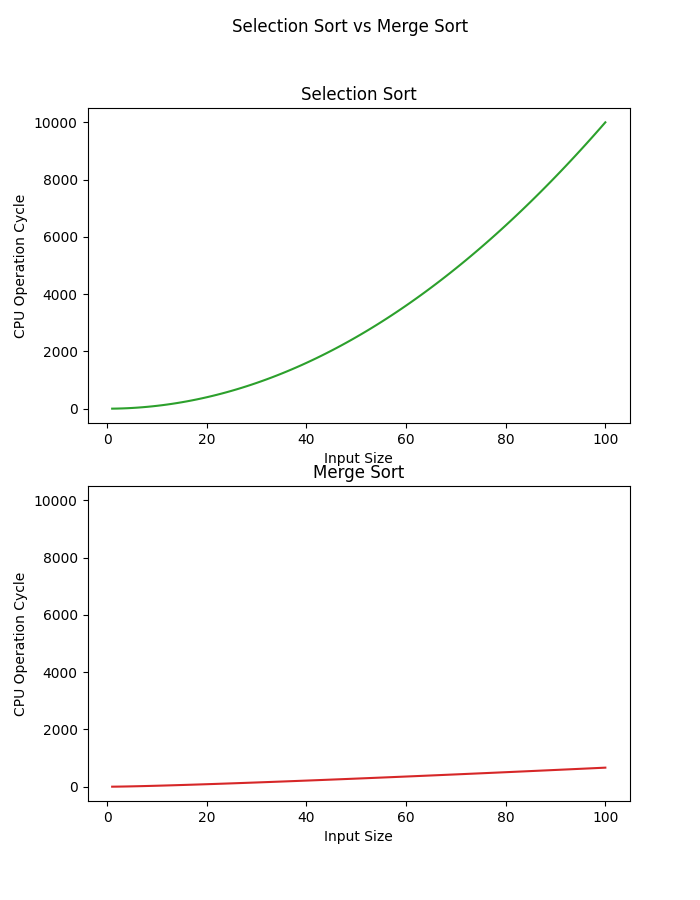
\includegraphics[width=7in,height=8.5in]{Selection Sort_Merge Sort.png}}
    \caption{Bubble Sort vs Merge Sort}
\end{figure}

\begin{figure}[h]
    \centerline{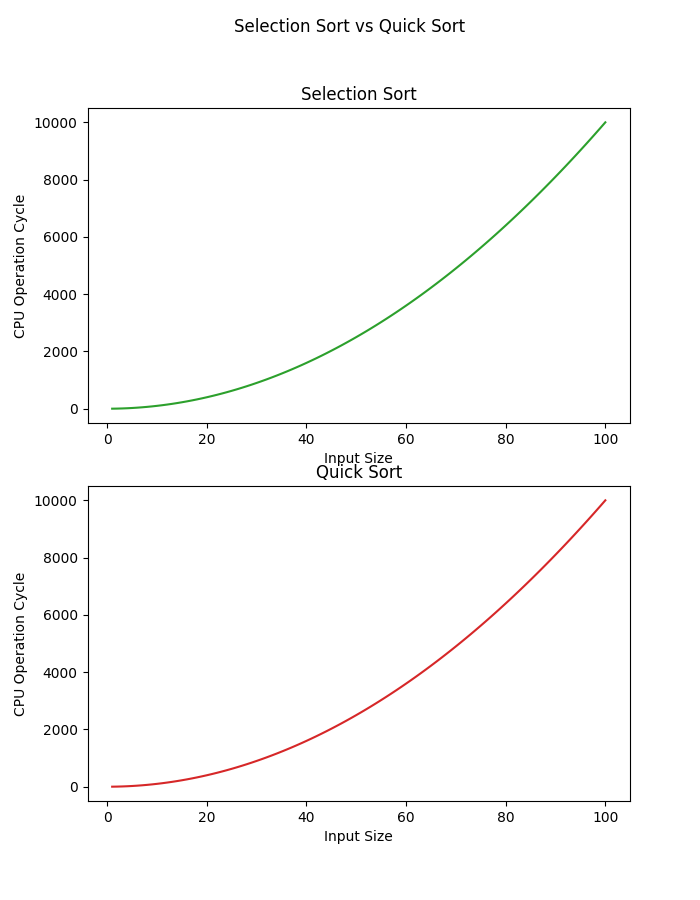
\includegraphics[width=7in,height=8.5in]{Selection Sort_Quick Sort.png}}
    \caption{Selection Sort vs Quick Sort}
\end{figure}

\begin{figure}[h]
    \centerline{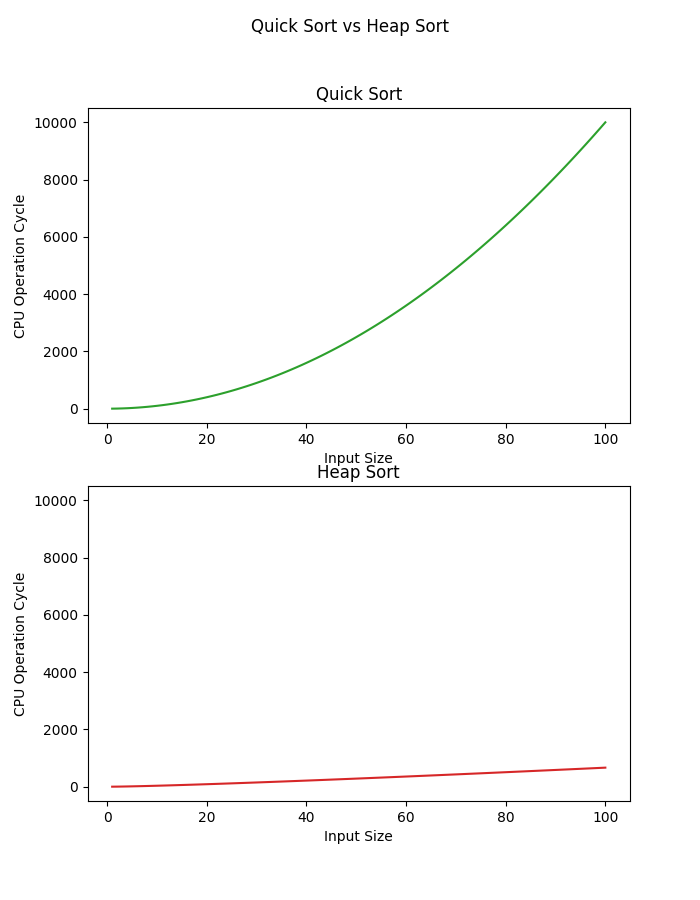
\includegraphics[width=7in,height=8.5in]{Quick Sort_Heap Sort.png}}
    \caption{Quick Sort vs Heap Sort}
\end{figure}
\end{document}
